\documentclass[../main]{subfiles}
\begin{document}
\chapter{Introducción}

La física estudia los componentes de la materia y sus interacciones, siendo estas las que explican las propiedades globales de la materia, así como los fenómenos que observamos en la naturaleza, intentando siempre dar forma matemática e interpretación a las leyes universales que rigen estos fenómenos. Por último aplicarlos en la solución de problemas y en proyectos preliminares de investigación.

Se verán los siguiente tópicos:

\begin{enumerate}
  \item Estructura atómica
  \item Física Estadística
  \item Estructura molecular
  \item Estado sólido
  \item Estructura nuclear
  \item Aplicaciones nuclear
  \item Partículas elementales
  \item Cosmología
\end{enumerate}

\section{Física Clásica}

\subsection{Mecánica newtoniana}

La materia se considera como un conjunto de partículas puntuales que se desplazan bajo la acción de las fuerzas de interacción mutua, segun las leyes de Newton.
\begin{align}
    F=\dot{p}=\frac{d}{dt}\left(mv\right)=\frac{dm}{dt}v+m\frac{dv}{dt}
\end{align}
A la materia se le considera como un conjunto de partículas de masa definida y el movimiento de cada partícula libre está caracterizado por su energía $\boldsymbol E$ y su impulso, $\boldsymbol p$.

\subsection{Mecánica analítica}

La materia se considera como en la newtoniana, pero es una teoría más elaborada que intenta eliminar los problemas de las ligaduras, el utilizar las magnitudes vectoriales y la dificultad de transición hacia la mecánica cuántica (un problema que tiene la mecánica newtoniana).

Las tres formulaciones más importantes son:

\begin{enumerate}
    \item \textit{Lagrangiana}, cuyas ecuaciones básicas son las ecuaciones de Lagrange.
    \item \textit{Variacional}, cuya ecuación básica es el principio de Hamilton.
    \item \textit{Hamiltoniana}, cuyas ecuaciones básicas son conocidas como las ecuaciones de Hamilton.
\end{enumerate}

\subsection{Teoría electromagnética}

Concierne a los fenómenos eléctricos y magnéticos que son descritos mejor en función de los campos eléctrico y magnética, $\boldsymbol{E}$($x$) y $\boldsymbol{B}$($x$).

Estos campos están relacionado con sus fuentes o causas, densidad de carga y densidad de corriente, mediante las ecuaciones de Maxwell.

En el espacio libre, los dos campos satisfacen la ecuación de ondas que en forma operacional es:
\begin{align}
    \left[\frac{1}{c^2}\frac{\partial^2}{\partial^2 x}-\nabla^2\right] \begin{Bmatrix}
\boldsymbol{E}(x)\\
\boldsymbol{B}(x)
\end{Bmatrix}=0,
\end{align}
estos campos se propagan en el espacio como ondas con una velocidad constante, $c$.

Ahora estamos familiarizados con otras formas de estas ondas electromagnéticas, desde las ondas de muy baja frecuencia utilizadas en radar y radioastronomía, pasando por el dominio de la luz, hasta las radiaciones de muy alta frecuencia de los rayos $X$ y rayos $\gamma$.

Gracias a la óptica geométrica, hay varias propiedades de la radiación para las que el concepto de onda no es esencial. No obstante, los fenómenos de interferencia y difracción son casos típicos donde la descripción ondulatoria es necesaria. La onda plana se expresa por:
\begin{align}
    \psi=\exp[-i(\omega t-\boldsymbol{k} \cdot \boldsymbol{x})],
\end{align}
donde $\omega$ es la pulsación y $\boldsymbol{k}$ es el vector de onda.

Dos características básicas de la onda, con $\omega=2\pi\nu$ y $\boldsymbol{k}=2\pi/\lambda$. La primera expresa la periodicidad temporal y la segunda, la especial.

Como la velocidad del grupo es $c$, ambas están relacionadas por:
\begin{align}
    \omega=kc
\end{align}
Estas dos disciplinas, mecánica y electromagnetismo, se acoplan mediante la \textit{ley de Lorentz}, expresión la dinámica de una carga $e$ de velocidad $\boldsymbol{v}$ en presencia de los campos $\boldsymbol{E}$ y $\boldsymbol{B}$.
\begin{align}
    \boldsymbol{F}(x)=e\left[\boldsymbol{E}(x) + \boldsymbol{v}\times\boldsymbol{B}\right]
\end{align}
Este cuadro del universo con la materia constituida de partículas puntuales (protones y electrones), y la \textit{radiación} constituida de ondas, podría haber suministrado el marco de una descripción fundamental de todos los fenómenos físicos. No obstante, los conceptos clásicos se mostraron completamente insuficientes para describir el movimiento de los electrones y su interacción.

\section{Insuficiencia de los conceptos clásicos}
\subsection{Aspectos de partícula de la radiación e hipótesis}
La primera indicación del fallo de los conceptos clásicos interviene en un fenómeno relativamente complicado, la radiación del \textit{cuerpo negro}, un problema termodinámico de intercambio de energía entre la radiación y la materia.

Clásicamente se creía que este intercambio de energía era continuo, es decir, que un foco luminoso puede ceder a la materia cualquier cantidad de energía según la intensidad. Planck en 1900 demostró que la ecuación termodinámica, que interpretaba correctamente las experiencias incluía la hipótesis de que el intercambio era discreto. Planck postuló que la radiación de pulsación $\omega$ solo puede intercambiar energía con la materia por cuantos de valor:
\begin{align}
    \hbar\omega=h\nu, \label{eq1}
\end{align}
donde además $\hbar=\cfrac{h}{2\pi}$.

Esta hipótesis significa que la radiación, en su interacción con la materia, se comporta como un haz de partículas (fotones) que puede ser emitido o absorbido por la materia. La energía en este caso está dado por:
\begin{align}
    E=h\nu,
\end{align}
donde además $h=6,62608\times10^{-34} J\cdot s$, también conocida como la \textit{constante de Planck}.

Como estos fotones se desplazan a la velocidad de la luz, según la teoría de la relatividad restringida su masa debe ser nula, 
\begin{align}
    E=mc^2,
\end{align}
reemplazando con la ecuación \ref{eq1}, la masa en movimiento es:
\begin{align}
    m=\frac{h\nu}{c^2}
\end{align}
y su momento lineal:
\begin{align}
    p=mc=\frac{h\nu}{c}.
\end{align}
También observamos que:
\begin{align}
    \begin{array}{r@{{}\mathrel{=}{}}c*{1}{@{{}\mathbin{+}{}}c}}
        E^2 & \underbrace{E^2_0} & (pc)^2 \\[\jot]
          &  \underbrace{m_0 c^2}  &  (pc)^2\\
          & 0 & (pc)^2\\
    \end{array}
\end{align}
Concluimos que $E=pc$, donde $\displaystyle p=\frac{hv}{c}=\hbar\frac{\omega}{c}=\hbar k$.

Podemos condensar nuestras conclusiones del siguiente modo:
\begin{align}
    E=\hbar\omega\\
    \boldsymbol{p}=\hbar \boldsymbol{k}
\end{align}
Estas ecuaciones son importantes pues muestran la relación entre los parámetros corpusculares ($E, \boldsymbol{p}$) del fotón y los parámetros ($w, \boldsymbol{k}$) de la onda correspondiente.
\begin{figure}[h]
    \centering
    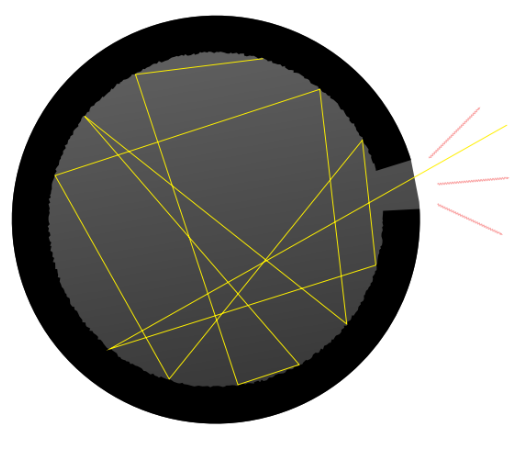
\includegraphics[width=6cm,height=6cm,keepaspectratio]{Física Moderna/General/img/1.png}
    \caption{Diagrama esquemático de un cuerpo negro}
    \label{fig:cuerpo_negro}
\end{figure}

\section{Conceptos importantes}
\subsection{Ley del desplazamiento de Wien}
Otto Fritz Franz Wien (1864-1928) logró demostrar que la longitud de onda $\lambda_{m\Acute{a}x}$, en la cual la densidad de flujo por intervalo unitario de longitud de onda que emerge del cuerpo negro es un máximo. Varía como:
\begin{align}
T\lambda_{m\Acute{a}x}=2,8978\times 10^{-3} m K    
\end{align}
\subsection{Ley de Stefan-Boltzmann}
La densidad de flujo radiante total o existencia es definida por:
\begin{align}
    M=\sigma T^4,
\end{align}
donde representa la constante de Stefan-Boltzmann:
\begin{align}
    \sigma=5,67\times 10^{-8} \frac{W}{m^2K^4}
\end{align}
\subsection{Distribución de Planck}
La densidad de energía en el rango entre $\lambda$ y $\lambda+d\lambda$ es dado por:
\begin{align}
    \text{d}E=\rho\cdot\text{d}\lambda, \label{eq3}
\end{align}
donde:
\begin{align}
    \rho=\frac{8\pi hc}{\lambda^5}\left(\cfrac{1}{e^{\displaystyle 
    hc/\lambda kT}-1}\right)
\end{align}
Esta expresión ajusta la curva experimental muy bien para toda longitud de onda y el valor de $h$ puede ser obtenido variando su valor hasta un mejor ajuste.
\begin{align}
    e^{\displaystyle hc/\lambda kT}-1&=\left[1+\cfrac{hc}{\lambda KT}+\cdots \right]-1\\
    &\approx \cfrac{hc}{\lambda KT}
\end{align}
Para longitudes de onda corta, $\displaystyle hc/\lambda kT$ es grande y $\exp(hc/\lambda kT)\rightarrow\infty$; por lo tanto:
\begin{align}
    \rho \rightarrow 0\text{, cuando }\begin{cases}
        \lambda \rightarrow 0\\
        \nu \rightarrow \infty
    \end{cases}
\end{align}
\subsubsection{Ley de Rayleigh-Jeans}
Partiendo de la ecuación \ref{eq3}:
\begin{align}
    E&=\int_0^\infty\rho\text{ d}\lambda\\
    &=aT^4,
\end{align}
donde $\displaystyle a=\frac{4\sigma}{c}$ y $\displaystyle \sigma=\frac{2\pi^5 k^4}{15c^2 h^3}$.

Un ejemplo del aspecto corpuscular de la radiación es:
\subsection{Efecto fotoeléctrico}
Propuesto por A. Einstein en 1905. Si un haz monocromático de pulsación $\omega$ incide sobre la superficie de un metal puede este emitir electrones. Si $\hbar\omega$ es inferior a un cierto límite $W$, llamado \textit{trabajo de extracción}, que depende del tipo de metal, no hay emisión para un amplio intervalo de intensidades de haz. Si $\hbar\omega > W$, los electrones son emitidos con una energía cinética $T$ tal que:
\begin{align}
    \hbar\omega = W + T
\end{align}
El efecto fotoeléctrico es una confirmación muy especial de la hipótesis de Planck, puesto que depende directamente del mecanismo de intercambio de energía, entre radiación y electrones, sin que intervengan otros efectos físicos.
\begin{align}
    E&=T_{m\Acute{a}x}+W_0\\
    h\nu&=T_{m\Acute{a}x}+h\nu_0\\
    h&=\cfrac{T_{m\Acute{a}x}}{\left(\nu-\nu_0\right)}\\
    T_{m\Acute{a}x}&=h\nu-h\nu_0
\end{align}
Además, $T_{m\Acute{a}x}=eV$, donde $e$ es la carga y $v$ es el potencial. El voltaje será entonces:
\begin{align}
    v=\cfrac{h(\nu-\nu_0)}{e}
\end{align}
\end{document}